%(BEGIN_QUESTION)
% Copyright 2006, Tony R. Kuphaldt, released under the Creative Commons Attribution License (v 1.0)
% This means you may do almost anything with this work of mine, so long as you give me proper credit

I følgende væske/damp-fylte system (Class II): hvor er væsken i systemet, og hvor er dampen i systemet?

$$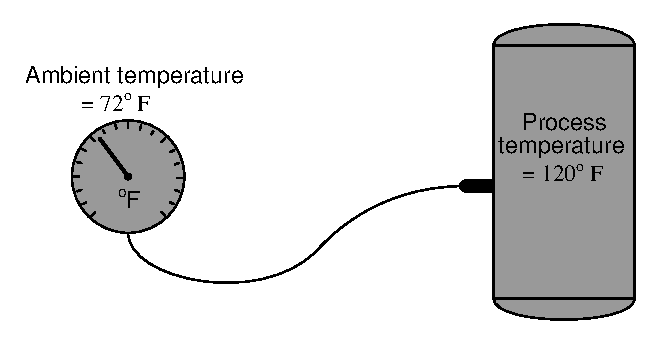
\includegraphics[width=15.5cm]{i00361x01.eps}$$

Hva skjer med plasseringen av væske og damp dersom prosesstemperaturen synker til 60$^{o}$ F?

\underbar{file i00361}
%(END_QUESTION)





%(BEGIN_ANSWER)

I scenarioet som er vist, vil væsken flytte seg mot den kaldere delen (indikatormekanismen), mens dampen flytter seg mot den varmere delen (bulb). Dette er typisk for Class II: væskedelen av fyllingen migrerer mot kald ende, dampdelen mot varm ende. Bare Class IID eliminerer dette problemet ved å bruke en ikke-flyktig væske som alltid fyller kapillar og måleelement (bourdonrør eller belg), slik at flyktig væske og damp holdes i bulben.

\vskip 10pt

Når prosesstemperaturen faller under omgivelsestemperaturen ved indikatorelementet (72$^{o}$ F), vil væsken forsøke å flytte seg mot bulben og dampen mot indikatoren. Under denne overgangen blir systemtrykket ustabilt, og temperaturmålingen blir uforutsigbar. Dette kalles ofte {\it cross-ambient}-problemet.

Av den grunn bør Class II unngås når prosessen kan ligge både over og under omgivelsestemperaturen ved indikatoren.

%(END_ANSWER)





%(BEGIN_NOTES)


%INDEX% Measurement, temperature: filled-bulb system

%(END_NOTES)
